\section{The catalogue}\label{sec:catalogue}

Tables~\ref{tab:catalogue} and~\ref{tab:catalogue2} list the claims, and Figure~\ref{fig:verdicts} shows them by verdict. The first column gives the claim in one line, in the form in which it was made; the second the paper in which it was made; the third the verdict; the fourth the section of this paper where the claim is examined and, where one exists, the theorem that settles it. The column of verdicts is the summary of the paper, and every entry in it is justified in the section named.\footnote{The format of the table, one claim per line with its source, its verdict and the place of the argument, is the barrier ledger of the engine Anaxia (\href{https://github.com/creelie/eBLLM}{\nolinkurl{github.com/creelie/eBLLM}}, release 3.1.0, \anaxiaDOIlink{}), described in \cite{BLLM26} and used in the same way for the records of \cite{Dwork26,YM26}. The engine was not run for this paper; only its ledger format is used.}

Three remarks on the choice of claims. First, the list contains every statement that Sen or his coauthors called a conjecture, every statement that was presented as a prediction for a regime not computed, and the main theorems whose proofs we have checked; it does not list the many papers that are computations within an established framework, since there is nothing to conjecture in them. Second, a statement that its author later corrected himself is not an error of the record and is not listed; the catalogue is of claims that stand in the literature as made. Third, the two statements recorded as \st{heuristic} are statements about regimes in which no quantity can be computed, and they are recorded for completeness and discussed in Section~\ref{ssec:matrix}, without a verdict.

\begin{table*}[t]
\centering
\footnotesize
\setlength{\tabcolsep}{4pt}
\renewcommand{\arraystretch}{1.08}
\begin{tabular}{@{}p{0.47\textwidth}p{0.17\textwidth}p{0.11\textwidth}p{0.19\textwidth}@{}}
\toprule
Claim & Source & Verdict & Where \\
\midrule
\multicolumn{4}{@{}l}{\textit{Duality}}\\
1. The heterotic string on $T^6$ is invariant under $SL(2,\ZZ)$ acting on the axion--dilaton & \cite{Sen94duality} & confirmed & \S\ref{ssec:sl2z} \\
2. The Atiyah--Hitchin manifold carries exactly one $L^2$ anti-self-dual harmonic two-form, the two-monopole bound state & \cite{Sen94dyon} & proved & \S\ref{ssec:twomonopole}, Thm~\ref{thm:atiyahhitchin} \\
3. The $L^2$ cohomology of the moduli space of $k$ monopoles, for every $k$, is as $S$-duality requires & \cite{Sen94dyon,SegalSelby96} & confirmed & \S\ref{ssec:senconjecture} \\
4. A manifestly duality-symmetric action is equivalent to the Maxwell and heterotic actions & \cite{SchwarzSen94} & proved & \S\ref{ssec:misc} \\
5. The rotating charged black hole of heterotic string theory is an exact solution & \cite{Sen92kerr} & proved & \S\ref{ssec:misc} \\
\multicolumn{4}{@{}l}{\textit{Quarter-BPS dyons}}\\
6. The dyon partition function of a CHL model is the inverse of a Siegel form with an explicit product formula & \cite{JatkarSen06,DJS06} & proved & \S\ref{ssec:chl} \\
7. Across a wall of marginal stability the index jumps by $(-1)^{Q\cdot P+1}|Q\cdot P|\,d_h(Q)\,d_h(P)$ & \cite{Sen07walls,Sen07twocentred} & proved & \S\ref{ssec:walls}, Thm~\ref{thm:wallcrossing} \\
8. Every state of negative discriminant is a two-centred bound state & \cite{Sen11negative} & proved & \S\ref{ssec:negative} \\
9. The index of a single-centred dyon is positive in every $\mathcal N=4$ compactification & \cite{Sen11positivity} & false as stated & \S\ref{sec:positivity}, Thm~\ref{thm:positivityfails} \\
10. The hair of a quarter-BPS black hole can be identified and removed, leaving a horizon index & \cite{BMS09hair} & confirmed & \S\ref{ssec:hair} \\
\multicolumn{4}{@{}l}{\textit{Tachyons on unstable branes}}\\
11. The tachyon potential of a D-brane is universal, independent of the background & \cite{Sen99univ} & proved & \S\ref{ssec:universality} \\
12. The tachyon vacuum has energy density $-\mathcal T_p$ relative to the brane & \cite{Sen98bab,Sen99nonBPS} & proved & \S\ref{ssec:threeconj} \\
13. Lower-dimensional D-branes are lump solutions of the tachyon effective theory & \cite{Sen98bab,Sen99nonBPS} & proved & \S\ref{ssec:threeconj} \\
14. There are no open string excitations around the tachyon vacuum & \cite{Sen99nonBPS,RSZ01} & proved & \S\ref{ssec:threeconj} \\
15. The three conjectures hold in the superstring field theory of Berkovits & \cite{BSZ00} & confirmed & \S\ref{ssec:threeconj} \\
16. The homogeneous rolling tachyon conserves energy and its pressure vanishes exponentially & \cite{Sen02rolling} & proved & \S\ref{ssec:homogeneous} \\
17. The final state of the decay of an unstable brane is tachyon matter, a pressureless dust & \cite{Sen02matter,Sen02field} & false as stated & \S\ref{ssec:caustic}, Thm~\ref{thm:caustic} \\
18. Open--closed duality at tree level: the open string description of the decay encodes the closed strings emitted & \cite{Sen03openclosed} & confirmed & \S\ref{ssec:emission} \\
19. The kink on a non-BPS D$p$-brane is the BPS D$(p-1)$-brane (descent relations) & \cite{Sen98spinor,Sen99descent} & proved & \S\ref{sec:nonbps} \\
20. Type I string theory has a stable non-BPS D-particle, the $SO(32)$ spinor & \cite{Sen98spinor} & proved & \S\ref{sec:nonbps} \\
21. The world-volume theory of the kink and the vortex is the Dirac--Born--Infeld action of the lower brane & \cite{Sen03kink} & proved & \S\ref{sec:nonbps} \\
\bottomrule
\end{tabular}
\caption{The catalogue, claims 1 to 21. ``Confirmed'' means that no proof exists and no test contradicts the claim; ``incomplete'' that the claim holds in the regime where it was derived and not in the regime to which it was extended; ``false as stated'' that there is a counterexample. Claim 36, in Table~\ref{tab:catalogue2}, is listed with the dyon claims it belongs to. Claims 9 and 17 are the two failures.}
\label{tab:catalogue}
\end{table*}

\begin{table*}[t]
\centering
\footnotesize
\setlength{\tabcolsep}{4pt}
\renewcommand{\arraystretch}{1.08}
\begin{tabular}{@{}p{0.47\textwidth}p{0.17\textwidth}p{0.11\textwidth}p{0.19\textwidth}@{}}
\toprule
Claim & Source & Verdict & Where \\
\midrule
\multicolumn{4}{@{}l}{\textit{F-theory}}\\
22. F-theory on an elliptic K3 has a weak coupling limit that is the type IIB orientifold on $T^2/\ZZ_2$ & \cite{Sen96ftheory} & proved & \S\ref{sec:senlimit} \\
23. The same limit exists for F-theory on an elliptic Calabi--Yau threefold, with D7-branes on a smooth divisor & \cite{Sen97orientifold} & incomplete & \S\ref{sec:senlimit} \\
\multicolumn{4}{@{}l}{\textit{Black hole entropy}}\\
24. The entropy function, extremised over the near-horizon data, gives the Wald entropy of an extremal black hole & \cite{Sen05entropy} & proved & \S\ref{ssec:entropyfunction} \\
25. The entropy function extends to rotating extremal black holes & \cite{AGJST06} & proved & \S\ref{ssec:entropyfunction} \\
26. The Gauss--Bonnet term reproduces the entropy $4\pi\sqrt{nw}$ of a small black hole in every dimension & \cite{Sen04stretch,Sen05stretching} & incomplete & \S\ref{ssec:small} \\
27. The quantum entropy function, a path integral over $AdS_2$, equals the microscopic index & \cite{Sen08qef} & confirmed & \S\ref{ssec:qef} \\
28. The logarithmic correction to the entropy is $0$ for $\mathcal N=4$ and $-4\ln A_H$ for $\mathcal N=8$ & \cite{BGMS11} & proved & \S\ref{ssec:logs} \\
29. For $\mathcal N=2$ the correction is $\tfrac{1}{12}(23+n_H-n_V)\ln(A_H/G_N)$ & \cite{Sen12N2} & confirmed & \S\ref{ssec:logs} \\
\multicolumn{4}{@{}l}{\textit{String field theory and other claims}}\\
30. Closed string field theory is background independent under infinitesimal deformations & \cite{SenZwiebach94} & proved & \S\ref{ssec:sft} \\
31. Superstring field theory has a gauge-invariant 1PI effective action and a BV master action, and is unitary & \cite{Sen15offshell,Sen15onePI,Sen16BV,Sen16unitarity} & proved & \S\ref{ssec:sft} \\
32. The normalisation of D-instanton amplitudes is fixed by string field theory & \cite{Sen20fixing,Sen21normalisation,Sen21IIB} & confirmed & \S\ref{ssec:instantons} \\
33. The classical logarithmic soft graviton terms are universal & \cite{LaddhaSen19,SahooSen19} & proved & \S\ref{ssec:soft} \\
34. The quantum logarithmic soft terms have the conjectured universal form & \cite{SahooSen19} & confirmed & \S\ref{ssec:soft} \\
35. A network of $(p,q)$ strings is a BPS configuration of type IIB & \cite{Sen98network} & proved & \S\ref{ssec:misc} \\
36. Every microstate of a single-centred BPS black hole carries zero angular momentum after the fermion zero modes are removed & \cite{CGMS16} & confirmed & \S\ref{ssec:hair} \\
H1. M-theory on $T^n$ is the large-$N$ limit of D0-branes on $T^n$ for every $n$ & \cite{Sen98matrix} & heuristic & \S\ref{ssec:matrix} \\
H2. For $n\ge 6$ the matrix description is a theory without an independent definition & \cite{Sen98matrix} & heuristic & \S\ref{ssec:matrix} \\
\bottomrule
\end{tabular}
\caption{The catalogue, continued: claims 22 to 36 and the two heuristic statements, which receive no verdict. Claims 23 and 26 are the two incomplete ones.}
\label{tab:catalogue2}
\end{table*}

\begin{figure}[t]
\centering
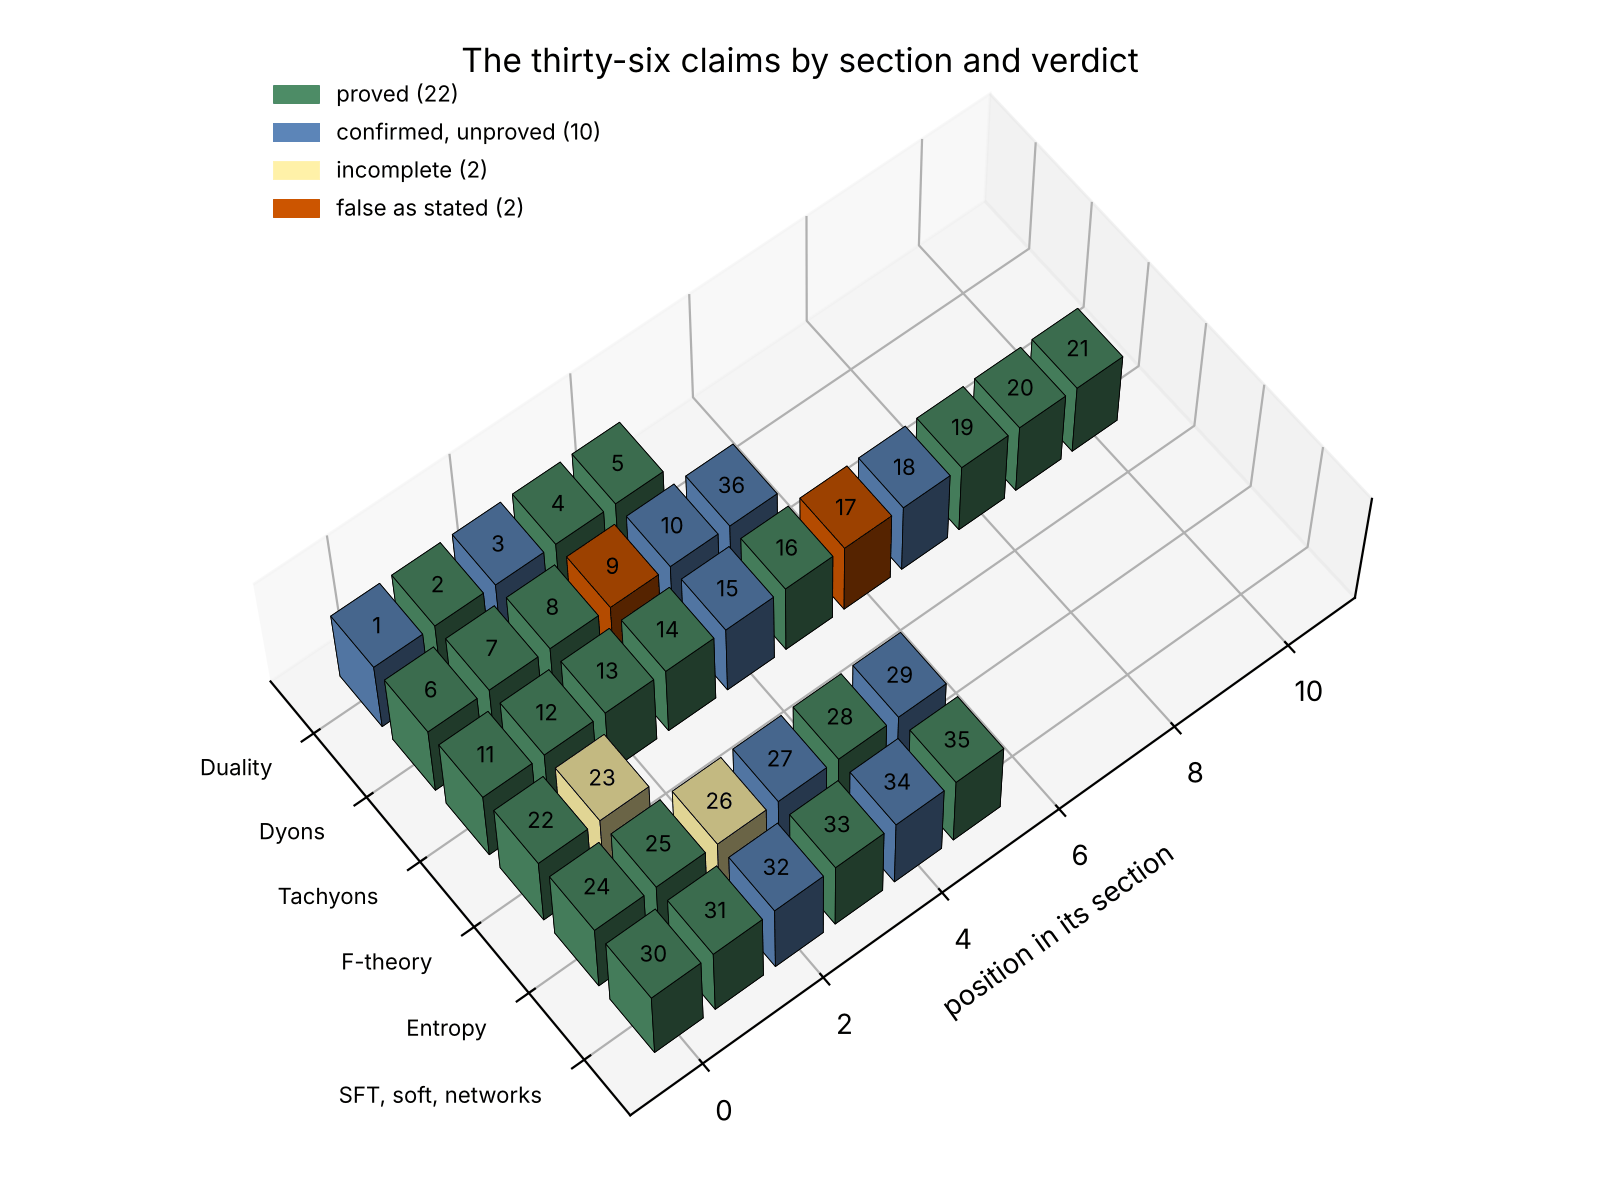
\includegraphics[width=\columnwidth]{figures/fig_verdicts.png}
\caption{The thirty-six claims of Tables~\ref{tab:catalogue} and~\ref{tab:catalogue2}, one block per claim, grouped by the section of the paper that treats them and coloured by verdict: proved, confirmed without proof, incomplete, false as stated. The two failures are claims 9 and 17; the two incomplete claims are 23 and 26.}
\label{fig:verdicts}
\end{figure}
